\section{Criando editatonas}

A fim de estudar a dificuldade de entrada de novos/as usuários/as \textit{in loco}, em nossa abordagem de pesquisa ``de fora para dentro'' resolvemos organizar nossas próprias editatonas como atividades de campo. Podendo assim observar problemas encontrados pelos/as participantes, e mapear com eles/as os mecanismos de governança da Wikipédia que se apresentam como barreiras, muitas vezes intransponíveis, deixando novatos/as bem intencionados/as sem saber como prosseguir.

Com isto, partindo das observações feitas \textit{in loco} nas editatonas, regressamos a bancada de ciência de dados de nosso laboratório. Nela andamos colados ao banco de dados, realizando inferências nos dados abertos da Wikipédia. Investigamos padrões, elementos e comportamentos da governança da comunidade que interagiram com nossos participantes durante e após as editatonas.

\subsection{Validando a escolha de realizar editatonas}

A metodologia adotada de realizar editatonas foi validada como pertinente logo no início da pesquisa em 2017, com a realização de uma atividade em sala de aula com a turma de pós-graduação da disciplina ``\textit{Estudos CTS (Ciências-Tecnologias-Sociedades): aproximações brasileiras e latino-americanas}'', ministrada no Programa de Engenharia de Sistemas e Computação da COPPE/UFRJ, no 2º período de 2017. Atividade esta que teve seus resultados retratados no trabalho ``\textit{Práticas de escrita biográfica na Wikipédia em português em turmas de pós-graduação}'', apresentado no VII Simpósio Nacional de Ciência, Tecnologia e Sociedade (Esocite.BR), também em 2017 (\cite{andrade_historias_2017}).

A editatona foi realizada durante uma aula em que o professor não poderia estar presente, e os/as estudantes deveriam se auto organizar e autogerir para realizar alguma atividade. Inicialmente o grupo imaginava que iria trabalhar no CTS Brasil Blog, site idealizado para escoar produções feitas ao longo do curso. Mas, no momento do encontro, percebeu-se que a produção deste já tinha seu fluxo de trabalho remoto bem definido, e que as horas que teríamos juntos presencialmente poderiam ser melhor aproveitadas de outra forma.

Assim, com a decisão de realizarmos uma editatona, o autor que vos escrever fez uma apresentação sobre o funcionamento da Wikipédia e suas políticas editoriais. Foi proposto então ao grupo que o escopo da atividade fosse o desenvolvimento de verbetes biográficos sobre os autores CTS que estavam sendo estudados na disciplina. O grupo então debateu sobre quais verbetes editar e, entendendo que existia um artigo que precedia os biográficos em importância para divulgação do tema CTS, definiu que seria feita uma força tarefa para melhorar apenas um verbete: ``\textit{Estudos de ciência, tecnologia e sociedade}''. Os 13 presentes então se dividiram em grupos, responsáveis por criar/melhorar diferentes seções do verbete em paralelo, que somadas comporiam a nova versão do verbete ao final da aula.

Antes da atividade, o verbete contava com 3.989 bytes\footnote{Unidade de medida utilizada pela comunidade para medir o tamanho de revisões e verbetes.}, distribuídos em uma breve introdução, uma seção textual intitulada ``Ensino'', seguida por seções de ``Bibliografia'' e ``Ligações externas''. Três horas depois, ao final da atividade, o texto já apresentava 23.570 bytes, sendo 20.281 bytes adicionados pela turma e 18 bytes adicionados pelo usuário FSogumo, que não era aluno do curso e adicionou, durante a atividade, o \textit{template} de geração automática de referências ao verbete, que agora contava com dez seções textuais diferentes.

Sabendo da dificuldade tão relatada de conteúdos criados em salas de aula persistirem por um longo período de tempo na Wikipédia (\cite{marques_trabalhando_2012}), (\cite{carver_assigning_2012}), (\cite{archuby_experiencias_2018}), (\cite{soler-adillon_wikipedia_2018}), voltamos então ao verbete ``\textit{Estudos de ciência, tecnologia e sociedade}'' um mês depois da realização da atividade, para pesquisar o que teria acontecido com as edições de nossos/as editores/as.

Encontramos mais três edições feitas por alunos da turma no verbete após a atividade, adicionando mais 10.551 bytes, e percebemos uma situação que contradiz toda a literatura sobre editatonas: nenhuma edição de nossa turma havia sido revertida, e todo o conteúdo criado por nossos/as novos/as editores/as continuava no ar. Este fato é ainda mais surpreende pois em nossa atividade os/as estudantes foram estimulados/as a editar diretamente a Wikipédia, sem realizar uso prévio das páginas de testes, o que diminuiria ainda mais as chances de sobrevivência de seus conteúdos (\cite{marques_trabalhando_2012}).

Perante tão distinta situação, resolvemos então investigar o que havia acontecido de especial em nossa editatona, e enredamos em nossa missão a ferramenta \textit{Objective Revision Evaluation Service} (ORES)\footnote{Em português Sistema Objetivo de Avaliação de Revisões.}, para analisar todas as edições feitas durante a atividade.

O ORES é uma ferramenta de inteligência artificial que avalia edições (também chamadas pelos/as usuários/as de revisões) feitas nas Wikipédias \citep{halfaker_artificial_2015}. Solicitamos aqui de nossos/as leitores/as a gentileza de aceitar o ORES como uma caixa-preta assim como ele é aceita pelos/as editores/as e reversores/as das Wikipédias\footnote{No uso cotidiano da enciclopédia o ORES faz parte das redes que sustentam outras caixas pretas que tomam decisões diretas ou apresentam relatórios, enquanto o ORES fica invisível fazendo suas avaliações no backend e seu nome permanece desconhecido para a maior parte da comunidade.}, e tomemos suas saídas como avaliações confiáveis sobre as edições apreciadas. Para cada edição avaliada, o ORES nos indica probabilidades dela ser danosa, feita em boa fé e de ser revertida (``apagada'').
\begin{center}
\begin{table}[hbt]
\begin{tabular}{ |c|c|c|c| } 
 \hline
\textbf{Id da Edição} & \textbf{Não danosa} & \textbf{Feita em boa fé} & \textbf{Deve ser revertida} \\
\hline
49529742 & 76\% & 87\% & 65\% \\
\hline
49529756 & 76\% & 90\% & 33\% \\
\hline
49529775 & 52\% & 59\% & 71\% \\
\hline
49529792 & 36\% & 35\% & 76\% \\
\hline
49529803 & 80\% & 84\% & 58\% \\
\hline
49529830 & 58\% & 61\% & 73\% \\
\hline
49529836 & 24\% & 34\% & 76\% \\
\hline
49529856 & 42\% & 56\% & 69\% \\
\hline
49531419 & 54\% & 63\% & 72\% \\
\hline
\textbf{49531652} & \textbf{98\%} & \textbf{99\%} & \textbf{04\%} \\
\hline
49781518 & 91\% & 96\% & 12\% \\
\hline
49785059 & 86\% & 88\% & 41\% \\
\hline
49802969 & 67\% & 88\% & 32\% \\
\hline
Média & 64\% & 72\% & 52\% \\
 \hline
\end{tabular}
\caption{Avaliação feita pelo ORES de todas as edições feitas na atividade, com a edição do coordenador da editatona destacada em negrito.}
\label{table:avaliacao-ores}
\end{table}
\end{center}
A tabela \ref{table:avaliacao-ores} exibe a avaliação do ORES para todas as edições feitas no contexto de nossa editatona, começando da mais recente e descendo cronologicamente. Observando a tabela podemos notar que a maioria de nossas edições foram percebidas pelo sistema como tanto feitas em boa fé como não danosas, mas apresentavam percentual alto de chances de serem revertidas.

Não por acaso, esse é exatamente o perfil de edição que organizadores de editatonas relatam vivenciar. Seus/suas colegas novatos estão editando em boa fé e realizando alterações que não são danosas para a enciclopédia, mas a falta de um determinado padrão de escrita, esperado pela comunidade, faz com que as edições sejam revertidas.

Ao observarmos atentamente a tabela criada pelo ORES uma edição nos salta aos olhos. A edição com id \textbf{49531652} apresenta 98\% de chances de não ser danosa, 99\% de ser feita em boa fé e apenas 4\% de chances de ser revertida. Ao clicar no detalhamento desta edição, podemos ver que ela havia sido feita pelo usuário experiente que coordenava a atividade (eu), e, nesta edição de 839 \textit{bytes}, todos os conteúdos criados nas edições anteriores eram revisados, sendo colocados no formato wikipédico, com ligações internas e referências organizadas no padrão wiki.

Esta edição específica, além de auxiliar a manter na enciclopédia os conteúdos que, segundo o ORES, tinham grandes chances de serem revertidos, estrutura o verbete e ajuda os próximos editores a criarem conteúdos mais ``aceitáveis'' para enciclopédia. As três edições seguintes a essa, feitas por alunos da turma, observam suas chances de serem revertidas caírem drasticamente. Antes da edição do coordenador da atividade, as edições dos novatos apresentavam em média 65,88\% de chances de serem revertidas. Já as realizadas por esse mesmo recorte de usuários/as posteriormente apresentam uma enorme queda nesse valor, para apenas 28,33\%.

Percebemos, então, a importância do coordenador da atividade não ser um mero tutor que orienta os participantes e apresenta políticas editorais e dicas de edição. Sua participação ativa na escrita coletiva dos mesmos verbetes que os/as editores/as novatos/as estiverem trabalhando pode auxiliar a manter as edições destes/as no ar, aumentando o sucesso da atividade tanto na satisfação dos participantes, como na disponibilização de mais conteúdos livres a longo prazo.

Seguindo o verbete ao longo dos meses, vimos que após a alta frequência de edições feitas pela turma em agosto e setembro de 2017, a página ``\textit{Estudos de ciência, tecnologia e sociedade}'' voltou a ser pouco editada. Nos dois anos seguintes, até o final de 2019, foram feitas apenas duas contribuições com adição substancial de conteúdo, que não dialogaram com o conteúdo criado pela turma, mas criaram uma seção sobre o ``movimento CTSA (Ciência, Tecnologia, Sociedade e Ambiente)''. Essas edições adicionaram 1415 bytes ao verbete, que permaneceram no ar não revisados nem contestados até o início de 2020.

Esse baixo volume de revisões no verbete mostra a importância das editatonas para não apenas apresentar o funcionamento da Wikipédia buscando engajar novos/as editores/as, como também para produzir conteúdos em assuntos que não sejam muito populares entre os/as editores/as habituais. Apesar de suas mais de 200 mil edições por mês, a Wikipédia tende a concentrar seu maior volume de edições em tópicos como política, esportes ou televisão.\citep{quarry_most_edited_pages_ptwiki_2019}

\begin{center}
\begin{table}[hbt]
\begin{tabular}{ |c|c| } 
 \hline
\textbf{Verbete} & \textbf{Edições em 2019} \\ 
\hline
Big Brother Brasil 19 & 581 \\ 
\hline
Governo Jair Bolsonaro & 357 \\ 
\hline
Copa São Paulo de Futebol Júnior de 2019 & 265 \\ 
\hline
Rompimento de barragem em Brumadinho & 247 \\ 
\hline
Primeira Liga de 2018–19 & 217 \\ 
\hline
Copa da Ásia de 2019 & 197 \\ 
\hline
Campeonato Mundial de Handebol Masculino de 2019 & 182 \\ 
\hline
Lista de participantes do Big Brother Brasil & 173 \\ 
\hline
Verão 90 & 168 \\ 
\hline
Temporada do Sport Club Corinthians Paulista de 2019 & 163 \\ 
 \hline
\end{tabular}
\caption{Lista de verbetes mais editados em 2019 na Wikipédia em português.}
\label{table:verbetes-mais-editados-2019}
\end{table}
\end{center}

Assim, conteúdos criados em editatonas que tenham como temática assuntos não midiáticos tendem a não receber muitas colaborações posteriores, e a produção gerada na atividade tenderá a se estabilizar como o conteúdo que futuros leitores terão acesso em suas pesquisas. Cabe dar bastante ênfase aqui ao fato de que, ao contrários de trabalhos científicos, que ``\textit{a maioria nunca é lida por ninguém}'' (\cite[p.59]{latour_ciencia_1987}), os artigos criados na Wikipédia tem uma grande audiência. E, quanto mais conteúdos tenha um verbete, mais facilmente ele será encontrado por robôs e indexado por mecanismos de busca, fazendo com que quanto maior ele esteja ainda mais leitores encontrem seu texto.

Com isso, quando uma editatona expande um verbete, além de estar melhorando a qualidade daquele conteúdo para a audiência previamente esperada, ela está também aumentando a audiência futura que terá acesso àquele verbete.

\begin{figure}[H]
    \centering
    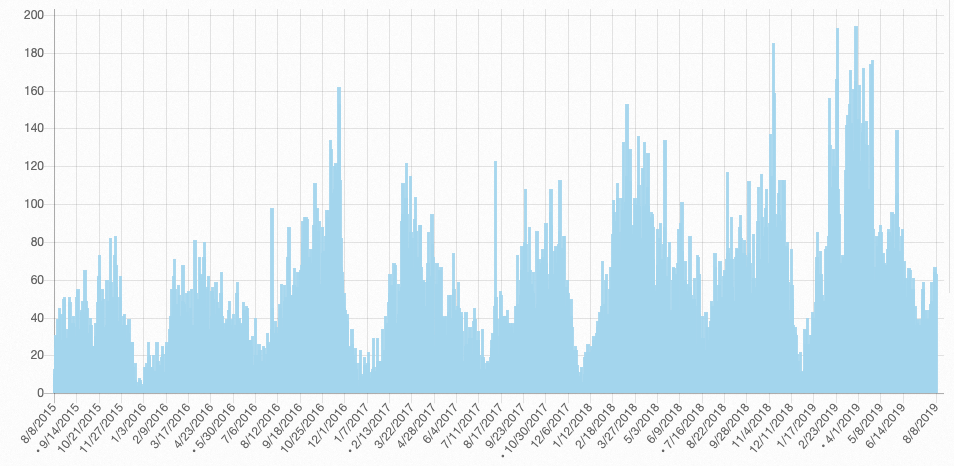
\includegraphics[width=1\textwidth]{Images/acessos-estudos-cts.png}
    \caption{Acessos ao verbete ``\textit{Estudos de ciência, tecnologia e sociedade}'' dois anos antes e dois anos depois da editatona.}
    \label{fig:acessos-estudos-cts}
\end{figure}

Na figura \ref{fig:acessos-estudos-cts} observamos os acessos ao verbete ``\textit{Estudos de ciência, tecnologia e sociedade}'' entre 8 de agosto de 2015 e 8 de agosto de 2019, exatamente dois anos antes e dois anos depois da editatona. Diferente do trabalho apresentado em 2017 (\cite{andrade_historias_2017}), que observara dois meses antes e dois meses depois da atividade, optamos por esse recorte maior de tempo para dar conta da sazonalidade observada nos acessos ao verbete ao longo do ano, que parece ser bastante influenciada pelo calendário escolar anual.

Compreendido então o recorde, observamos que, nos dois anos anteriores à editatona, o verbete apresentava uma audiência média de 38 acessos por dia. Nos dois anos seguintes, esse número cresce 55,26\%, para 59 acessos diários.

Em valores absolutos, e considerando que o verbete manteria um volume estável de visitas com seu conteúdo anterior\footnote{Consideração benevolente, pois entre 2016 e 2019 os acessos à Wikipédia em português como um todo caíram 1,5\%\citep{wikimedia_stats_page_views_ptwiki}}, isso significa que a editatona de 3 horas, com 13 participantes, proporcionou em dois anos 15.330 leituras a mais sobre ``Estudos de ciência, tecnologia e sociedade'' em português.

Perante o volume de acessos da Wikipédia, aproximadamente 13 milhões por dia somente em português\citep{wikimedia_stats_page_views_ptwiki}, essas 15 mil leituras em dois anos podem parecer poucos relevantes. Mas, dentro de seu nicho específico de um assunto não muito midiático como ``Estudos de ciência, tecnologia e sociedade'', esse número significa que, no mundo real, 15 mil pessoas que antes não teriam encontrado esse conteúdo em português sobre o tema agora o terão, e em uma versão do texto enciclopédico com maior abrangência e mais referências do que eram apresentadas antes da editatona.

A título de comparação da relevância deste volume de acessos, podemos olhar para os números de outra atividade desenvolvida pela mesma turma: o ``CTS Brasil Blog''\footnote{Disponível em https://ctsbrasilblog.wordpress.com/ .}. Ao longo de todo o curso, os/as estudantes criaram conteúdos e os publicaram nesta página, dedicada especialmente a ``\textit{circular vídeos, resenhas, entrevistas, manifestos e o que mais sair das digestões feitas durante a disciplina}'' (\cite{cts_brasil_blog}). Ao final do curso, o site contava com 17 publicações, feitas por 10 autores/as diferentes.

No ano de sua criação o blog teve seu pico de acessos, muito provavelmente ocasionado pelas visitas dos/as próprios/as estudantes-autores, com 526 visitas em 2017. No ano seguinte, este número cai para 215 e, em 2019, o blog encerra o ano com 149 visualizações. Enquanto o volume de acessos inicial pode ser explicado pelos autores acessando o site durante a disciplina, pois nos dois primeiros meses de vida enquanto a disciplina acontecia o \textit{site} recebeu 482 visualizações, os meses seguintes de novembro e dezembro somados totalizam 44 visitas. Podemos então considerar que em outubro de 2017 o blog é estabilizado por seus/suas autores/as, que param de publicar após o término da disciplina, e que os acessos que acontecem a partir daí seriam feitos por leitores/as alheios ao curso. Assim, considerando todos os acessos dos dois últimos meses de 2017 e os anos inteiros de 2018 e 2019, no que podemos considerar leituras orgânicas\footnote{Em mídias sociais, esse é o termo utilizado para acessos feitos sem pagamento de divulgação, por usuários que encontram o site através de links externos ou buscadores.} do conteúdo, temos um volume de 408 visualizações, em uma média de 0.51 visitas por dia.

\begin{figure}[H]
    \centering
    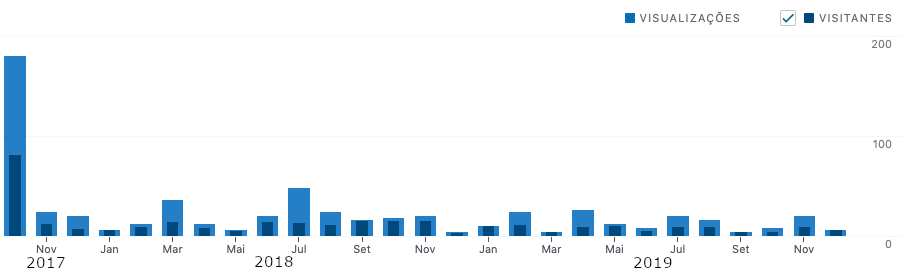
\includegraphics[width=1\textwidth]{Images/acessos-cts-brasil.png}
    \caption{Acessos ao CTS Brasil Blog por mês.}
    \label{fig:acessos-cts-brasil}
\end{figure}

Essa iniciativa do CTS Brasil Blog é claramente um caso de sucesso de divulgação científica, que continua no ar até hoje apresentando para leitores lusófonos, e em grande maioria do Brasil (89,3\%, como pode ser visto na figura \ref{fig:acessos-geo-cts-brasil}), conteúdos sobre os Estudos de Ciências-Tecnologias-Sociedades que outrora ficariam restritos às salas de aula de pós-graduação. Mas, seu relevante volume de acessos parece pequeno se comparado às mais de 15 mil visitas que receberam os conteúdos criados na editatona realizada pela mesma turma.\footnote{É importante destacar que o blog aceitava diferentes tipos de conteúdos, e não apenas textos enciclopédicos. Aqui comparamos seus acessos não para medir qual atividade teve maior sucesso, mas apenas para colocar o alcance da atividade realizada na Wikipédia em perspectiva.}

\begin{figure}[H]
    \centering
    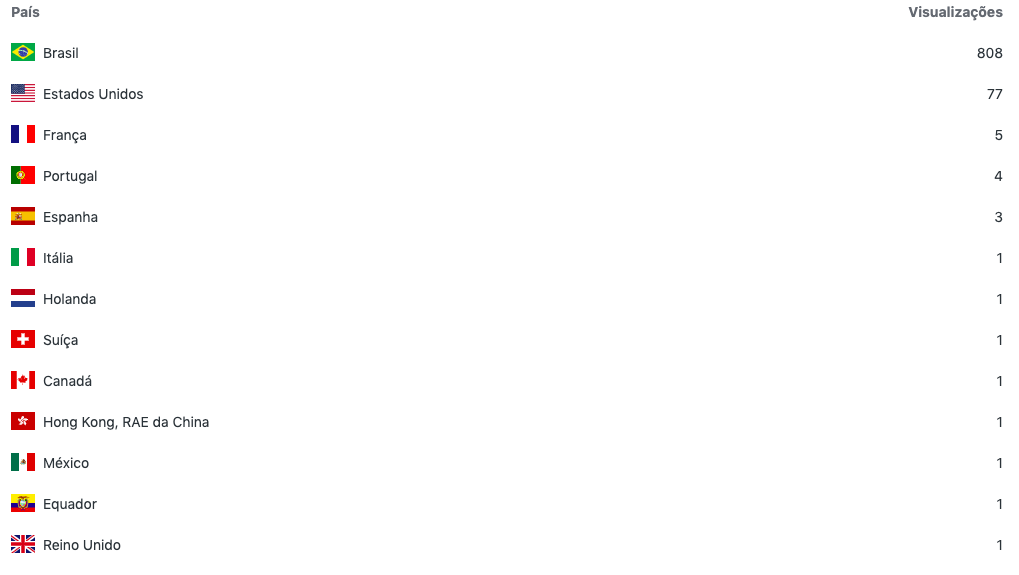
\includegraphics[width=1\textwidth]{Images/acessos-geo-cts-brasil.png}
    \caption{Acessos Geolocalizados ao CTS Brasil Blog.}
    \label{fig:acessos-geo-cts-brasil}
\end{figure}

Tendo em mente estes casos de sucessos na criação de conteúdos, que são de fato lidos pela sociedade além dos muros da universidade, decidimos que procederíamos com a realização de mais editatonas no curso da pesquisa, e convidaríamos para participar das atividades as redes que orbitam o Laboratório de Informática e Sociedade (LabIS) da COPPE/UFRJ, fazendo com que nosso trabalho de campo tenha um efeito colateral um tanto quanto interessante: enquanto estudamos os mecanismo de entrada de novatos na Wikipédia, criamos conteúdos livres em português sobre assuntos relacionados a Ciências-Tecnologias-Sociedades locais, tais como moedas sociais, softwares para acessibilidade, educação popular, informática e educação, mobilização política em redes sociais e demais assuntos que interessarem aos participantes das atividades. Promovemos assim maior acesso de leitores/as do idioma português, por todo o mundo, a esses conteúdos muitas vezes ignorados nos meios de divulgação científica e marginalizados por grande veículos de comunicação.

\subsection{Preparando nossa série de editatonas}

Nossa pesquisa avança então como objetivo organizar editatonas presenciais para tanto acompanhar \textit{in loco}, com o olhar míope da formiga, como acontecem as interações entre novatos e enciclopédia, como também para disponibilizar livremente em páginas bastante visitadas conteúdos sobre assuntos relacionados a pesquisas do campo CTS e correlatos.

Nos preparativos para a realização destas editatonas estudamos o histórico das diversas editatonas já realizadas pelo movimento Wikimedia, performando uma extensa revisão bibliográfica dos chamados Learning Patterns da comunidade Wikimedia. A comunidade Wikimedia mantém uma instalação do MediaWiki chamada Meta, onde as páginas pode ser utilizadas para planejar atividades, acompanhar projetos e compartilhar aprendizados. \citewiki{meta_home_page} Uma das áreas mais populares desta wiki são os Learning Patterns, onde wikimedistas são estimulados a compartilhar de forma estruturada rotinas padronizadas que foram aprendidas e podem replicadas por outros extensionistas wikipedistas. Como explicado por Erick Moeller, Deputy Director da Wikimedia Foundation em 2009, ``nossa iniciativa de outreach está desenvolvendo um conjunto abrangente de materiais de treinamento e divulgação que nos ajudarão a recrutar novos editores voluntários.'' \citep{moeller_wikipedias_2009}\footnote{Tradução livre do inglês: ``\textit{Our outreach initiative is developing a comprehensive set of training and outreach materials that will help us to recruit new volunteer editors.}''}

\begin{figure}[H]
    \centering
    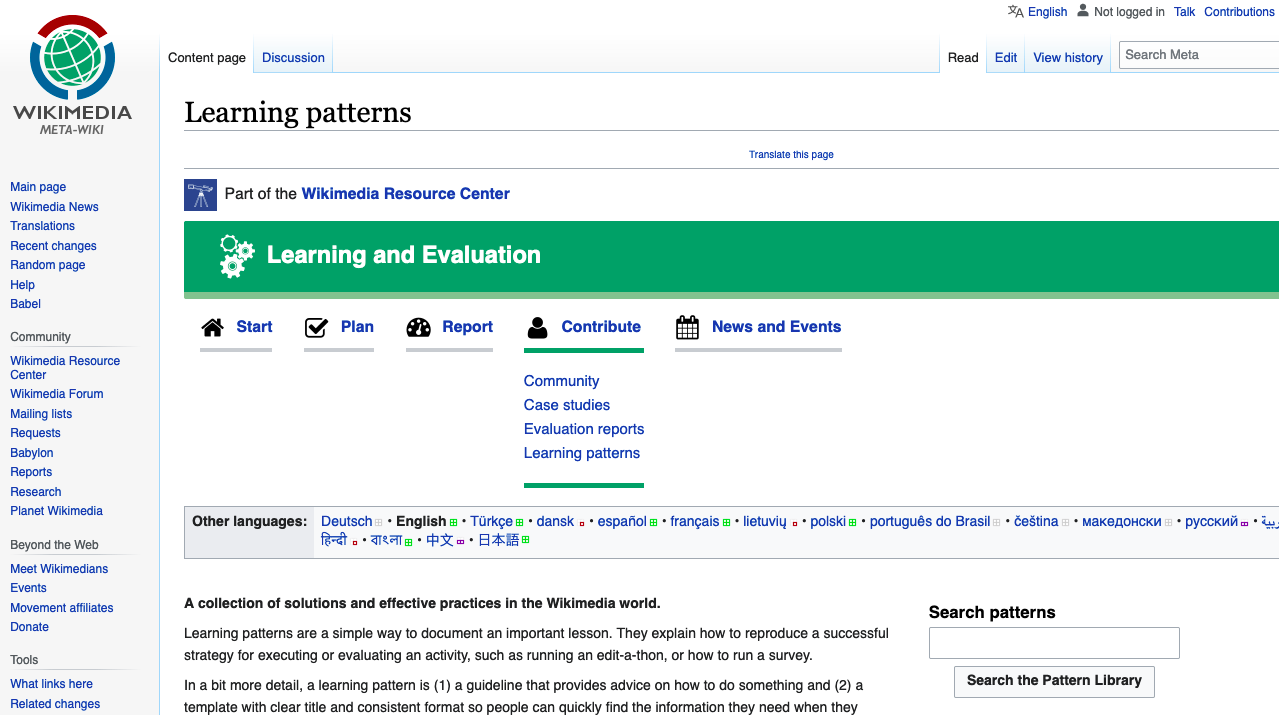
\includegraphics[width=1\textwidth]{Images/learning_patterns.png}
    \caption{Portal de Learning Patterns do movimento Wikimedia.}
    \label{fig:learning_patterns}
\end{figure}

Cabe aqui fazer uma ressalva de que em nossa pesquisa entendemos como o conceito de ``melhores práticas'', remetido pelos \textit{learning patterns} é problemático. Pois afinal ``toda prática é surpreendente'' \citep{cukierman_pasteur_2007} e especificidades locais e temporais jamais poderão ser em sua totalidade capturadas por guias e manuais. No entanto, essa preocupação não significa que devamos descartar todo conhecimento produzido em outros contextos. Buscamos as ``\textit{melhores práticas}'' da comunidade global na organização de editatonas para termos um ponto de partida, que necessariamente seria adaptado para a realidade de nossas atividades (e como o leitor saberá nas próximas sessões, essas adaptações para nossa realidade foram ainda mais intensas e numerosas do que havíamos antecipado).

Dentre os mais de 400 learning patterns disponíveis na wiki Outreach no momento de nossa pesquisa elegemos 13, que versam explicitamente sobre a realização de editathona para serem estudados a fundos e utilizados como inspiração para criação do roteiro para as nossas editatonas. Os learning patters escolhidos para serem nosso ponto de partida foram desde alguns mais genéricos sobre a realização das ativdades, como ``How to make editathons for new users more successful'' \citewiki{meta_how_to} e ``New users are afraid of doing something wrong'' \citewiki{meta_new_users} até outros mais específicos como ``Six-account limit'' \citewiki{meta_six_account} e ``Capturing User names at workshops'' \citewiki{meta_capturing_usernames}. 

\subsubsection{Criando nosso roteiro}

Seguindo as lições aprendidas com os learning patterns estudados, criamos um roteiro prevendo ações a serem realizadas antes, durante e depois de cada editatona. 

** Sobre a criação do roteiro https://trello.com/c/dH13LfQh/466-detalhar-a-cria%C3%A7%C3%A3o-do-meu-roteiro-da-organiza%C3%A7%C3%A3o-de-uma-editatona

\subsubsection{Criando artefatos para o roteiro funcionar}

Para darmos conta de todas as preocupações elencadas e alcançarmos os objetivos da atividade, foram criados alguns artefatos em forma de predefinições da Wikipédia.

Predefinições são página do MediaWiki que funcionam como templates, podendo ser importadas para outras páginas trazendo automaticamente uma estrutura previamente determinada. Nossas predefinições foram criada para facilitar a utilização das páginas de testes pelos participantes das editatonas. Estas predefinições permitiram com facilidade a criação e listagens de novas subpáginas de testes, tarefa mapeada como complexa nos learning patterns por não ser nada trivial para um usuário não habituado ao funcionamento do MediaWiki.

Foram criadas três predefinições, que estão publicamente disponíveis na Wikipédia para ampla utilização. 

Partindo do pressuposto de que o editor recém chegado à Wikipédia deseja produzir conteúdo, e somente após se engajar na ``atividade-fim'' da comunidade poderá talvez desenvolver interesse pelas ``atividades-meio'', como a estrutura do MediaWiki, planejamento a criação das nossas pré-definições de forma a ``tornar invisível'' para o entrante toda essa complexidade, e facilitar seu foco na produção de conteúdo.

\begin{figure}[H]
    \centering
    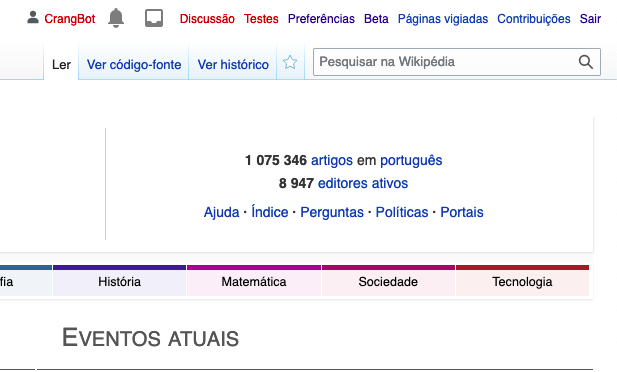
\includegraphics[width=1\textwidth]{Images/link_testes_vermelho.png}
    \caption{Link para página de testes vermelho, indicando que página não existe.}
    \label{fig:link_testes_vermelho}
\end{figure}

Com isso em mente, foi criada a pré-definição ``Predefinição:Página de testes do usuário'', que em nosso roteiro deve ser incluída pelo coordenador da editatona na página de testes de cada participante tão logo ele se identifique. Desta forma, acontecerão duas coisas: (1) o link no menu superior do MediaWiki para ``testes'' deixará de ser vermelho (indicação de uma página inexistente) para ser azul (mais convidativo ao clique) e (2) quando o usuário clicar em ``testes'', ele não se defrontará simplesmente com uma página em branco, mas sim com o mais amigável conteúdo que pode ser visto na \ref{fig:pagina_de_testes_editatona}.

\begin{figure}[H]
    \centering
    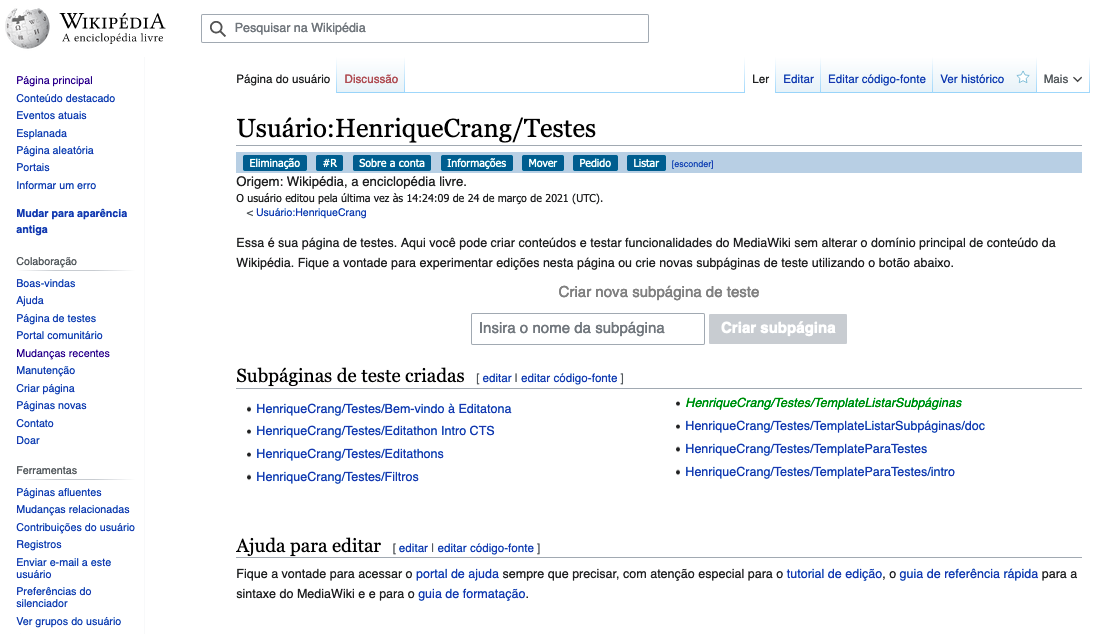
\includegraphics[width=1\textwidth]{Images/pagina_de_Testes.png}
    \caption{Página de testes criada utilizando as predefinições desenvolvidas pela pesquisa.}
    \label{fig:pagina_de_testes_editatona}
\end{figure}

A nova página de testes do usuário, criada a partir de nossa predefinição apresenta quatro seções: (1) uma breve explicação sobre o que é a página de testes, (2) um botão para facilitar a criação de uma nova subpágina de testes, (3) uma lista de todas as subpáginas de testes criadas por aquele usuário e (4) links para as páginas onde o usuário pode encontrar guias tutoriais e demais materiais que o auxiliem a editar.

A primeira sessão é autoexplicativa, então partimos para explica a segunda: ``Criar nova subpágina de teste ''. Na estrutura do MediaWiki é comum a criação de ``subpáginas'', especialmente em suas areas administrativas. Para criar uma página que seja ``subbalterna'' a outra, é necessário acessa a URL da futura página, ou a procurar na ferramenta de busca do MediaWiki. Essa geração de nova página deve ser feita adicionando o nome da página ``mãe'' seguido de uma ``/'' e do nome da subpágina. Como exemplo, poderíamos ter ``Página/Subpágina''.

Uma vez acessado o endereço da futura nova página, o MediaWiki informa ao usuário que ela ainda não existe, e oferece ao usuário a opção de iniciar uma página nova (como pode ser visto na \ref{fig:criacao_pagina_url}). 

\begin{figure}[H]
    \centering
    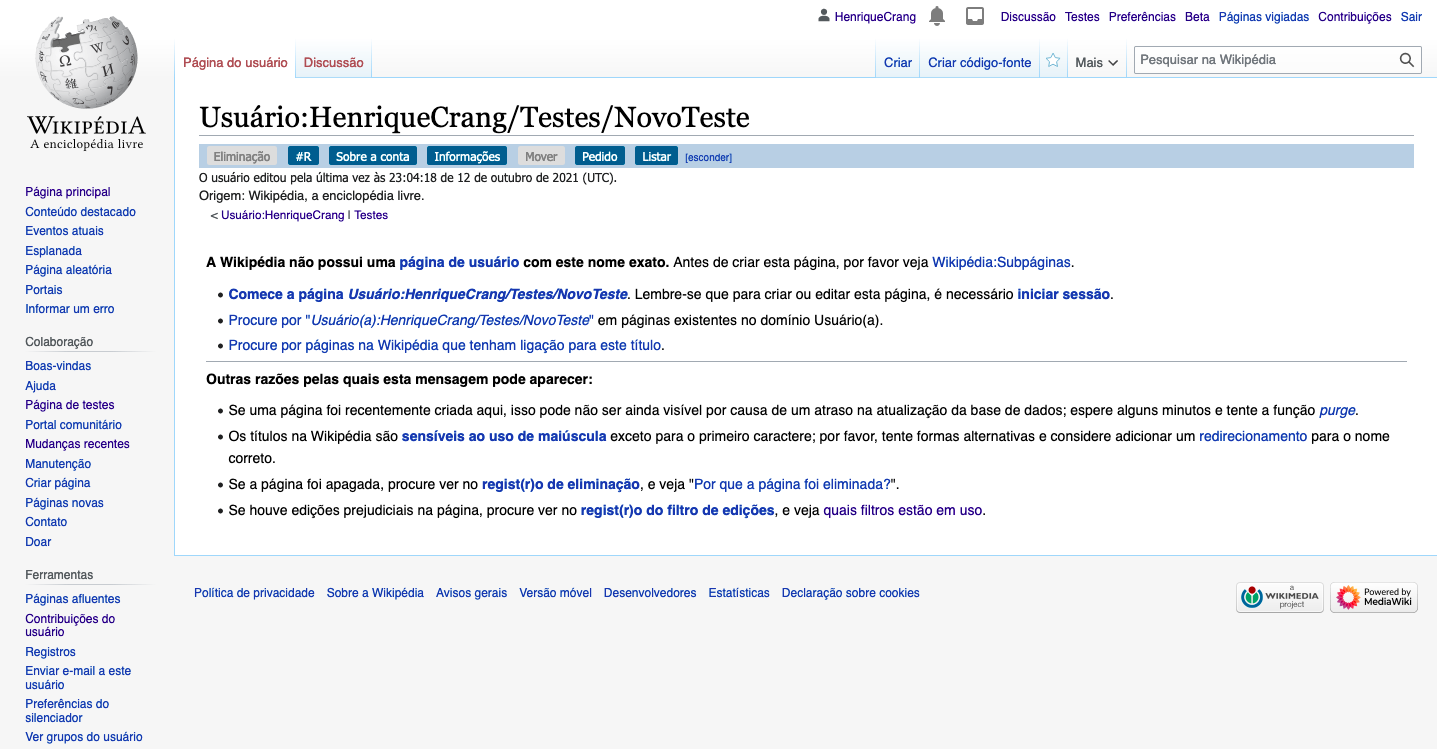
\includegraphics[width=1\textwidth]{Images/criacao_pagina_url.png}
    \caption{Endereço de futura página de testes sendo acessado diretamente pela URL.}
    \label{fig:criacao_pagina_url}
\end{figure}

Esse processo aparentemente simples para quem já o conhece é um tanto quanto difícil de ser explicado e nada intuitivo para quem está fazendo pela primeira vez. Para aumentar a complexidade da compreensão desta árvore de subpáginas pelos novatos, caso ele deseje criar mais de uma página de testes, é recomendado que as novas páginas sejam subpáginas da subpágina de testes. Assim, seguindo o exemplo de meu usuário, uma nova página de testes poderia se chamar ``Usuário:HenriqueCrang/Testes/Novo\_Teste''.

A fim de facilitar esse processo, foi criado um campo onde o usuário informa o nome desejado para criar uma nova subpágina e um botão que irá o levar diretamente para a area de edição desta nova página, economizando assim um passo neste processo de criação e facilitando o caminho do editor.

\begin{figure}[H]
    \centering
    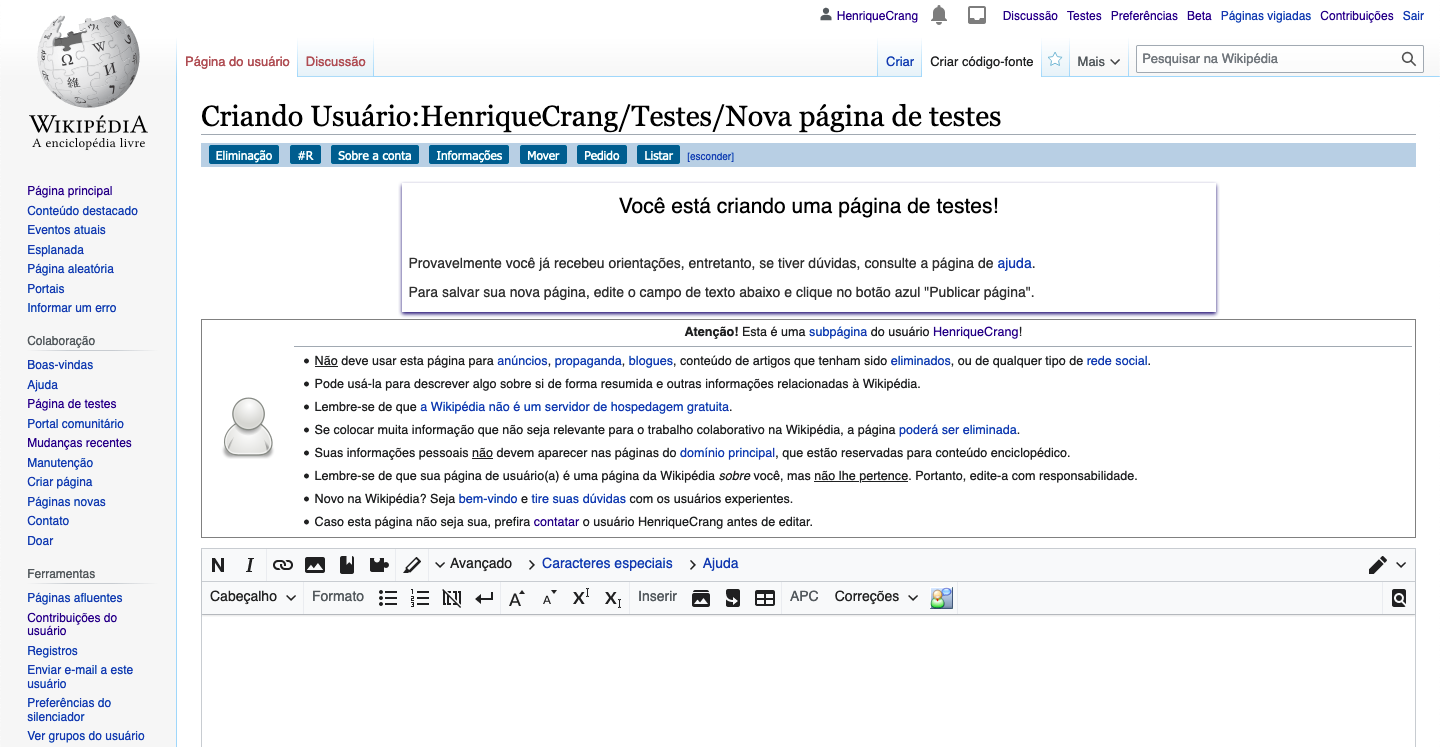
\includegraphics[width=1\textwidth]{Images/criacao_pagina_com_template.png}
    \caption{Página de testes sendo criada através de nossa predefinição, com a caixa de aviso mais amigável.}
    \label{fig:criacao_pagina_com_template}
\end{figure}

Na figura \ref{fig:criacao_pagina_com_template} podemos ver uma subpágina nova sendo criada a partir de nosso botão. Aproveitando que o código de nossa predefinição está criando esta nova página, aproveitamos para adicionar a ela uma nova caixa informativa chamada ``Você está criando uma página de testes!'', dando destaque ao usuário para em que momento do processo ele se encontra e oferecendo um link para a página de ajuda. O conteúdo desta caixa informativa mais amigável é importado de outra predefinição criada por nós, chamada ``Predefinição:Página de testes do usuário/intro''.

\begin{figure}[H]
    \centering
    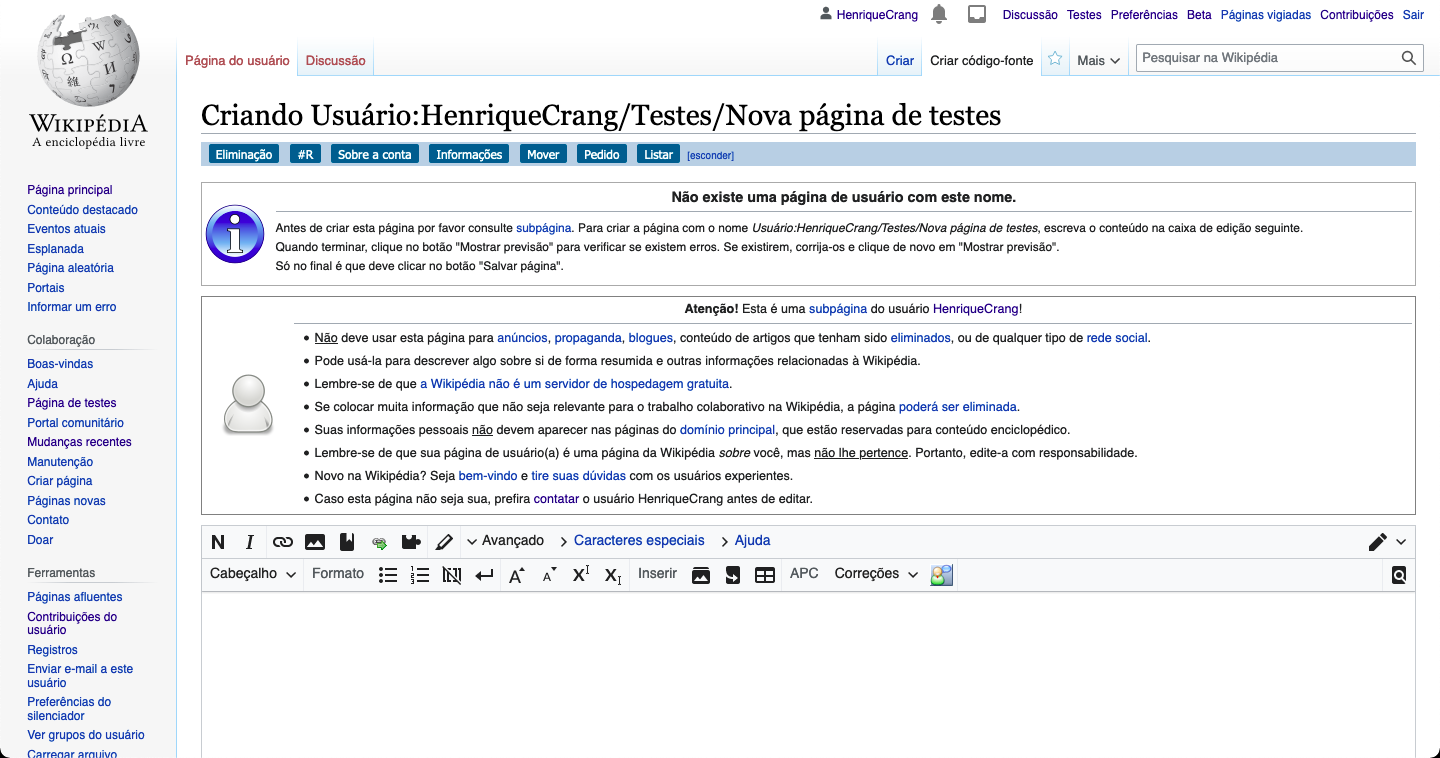
\includegraphics[width=1\textwidth]{Images/criacao_pagina_sem_template.png}
    \caption{Página de testes sendo criada sem utilizar nossa predefinição.}
    \label{fig:criacao_pagina_sem_template}
\end{figure}

A terceira sessão da página de testes criada pela predefinição das nossas editatonas contém uma lista de subpáginas de testes criadas por aquele usuário, facilitando seu acesso futuro e navegação entre elas. Para que essa lista fosse gerada, criamos uma outra predefinição chamada ``\textit{Predefinição:Listar subpáginas}'', que adicionará onde for incluída uma lista com todas as subpáginas da página. 

A listagem de subpáginas é especialmente importante para as editatonas pois as páginas de testes são subpáginas da página de cada usuário. Como exemplo, a página de meu usuário pode ser acessada em ``Usuário:HenriqueCrang'' enquanto minha página de testes padrão em ``Usuário:HenriqueCrang/Testes''.

E não é nada trivial conseguir posteriormente listar as subpáginas de uma determinada página. Umas das formas de fazer isso é buscando pelo nome da página "mãe" na ferramenta de buscas do MediaWiki. Porém, caso a página mãe tenha sido mencionada em qualquer outra página, esta outra também aparecerá no resultado da busca, poluindo o resultado da pesquisa.

Existe uma grande complexidade nesta a princípio simples ação de encontrar as subpáginas criadas, que apresenta uma íngreme curva de aprendizado sobre o funcionamento do MediaWiki a ser vencida para que a navegação por elas aconteça. E, definitivamente, esta não é a lição mais divertida para ser ensinada a um novato, que está mais interessado em ter acesso direto aos espaços de escrita. Assim, nossa predefinição oferece aos entrantes uma forma rápida e fácil de acessar seus conteúdos em desenvolvimento.

Chegamos então a quarta e última sessão de nossa repaginada página de testes que, apesar de simplória, apresentando apenas a frase ``\textit{Fique a vontade para acessar o portal de ajuda sempre que precisar, com atenção especial para o tutorial de edição, o guia de referência rápida para a sintaxe do MediaWiki e e para o guia de formatação.}'' acreditamos ser de grande importância. Uma das grandes reclamações relatadas por entrantes na Wikipédia é a dificuldade de encontrar informações sobre como editar corretamente. Seja informações sobre como utilizar o Markdown do MediaWiki ou como enviar um pergunta para um usuário mais experiente, esses espaços para serem encontrados demandam um certo conhecimento da operação da plataforma e da estruturação de conteúdos em uma wiki, coisas que normalmente um novato média não tem. Assim, nesta sessão agrupamos quatro links internos para areas da Wikipédia mais apropriadas para novatos encontrarem dicas e pedirem ajuda.

Centralizando todas essas informações na página de testes do usuário, temos como expectativa que ela passe a ser utilizada como o ``ponto de partida'' do usuário a cada vez que for editar, o auxiliando tanto na criação de seus testes como na obtenção de ajuda e tornando a experiência de começar a editar a Wikipédia mais agradável.

\subsection{Colocando o plano em prática}

***  Falar aqui da primeira editatona, feita presencialmente em 21 de novembro de 2019.

https://pt.wikipedia.org/wiki/Wikip%C3%A9dia:Edit-a-thon/Atividades_em_portugu%C3%AAs/Editathon_ECI_UFRJ

\begin{figure}[H]
    \centering
    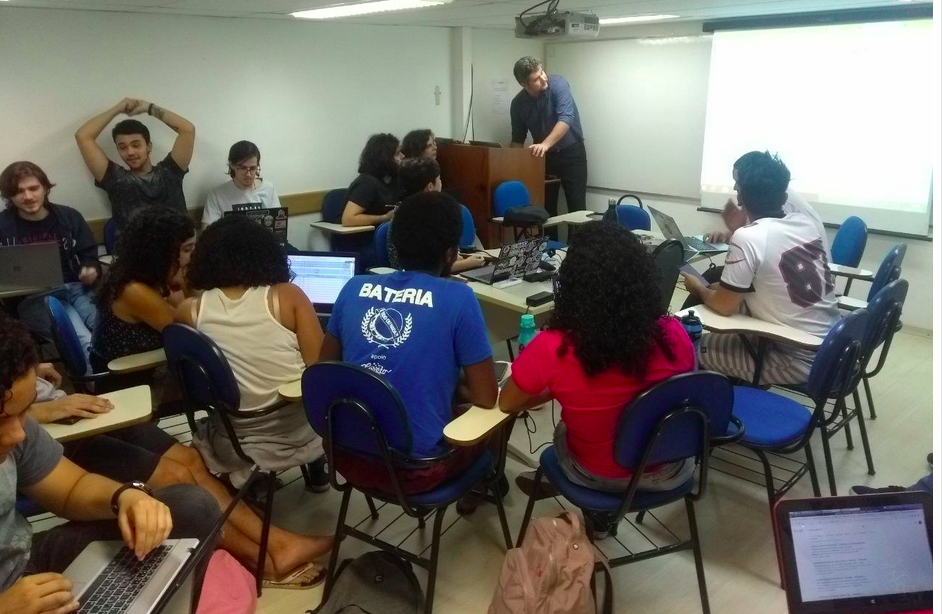
\includegraphics[width=1\textwidth]{Images/editatona_presencial.png}
    \caption{Editatona presencial com turma de graduação realizada no dia 21 de novembro de 2019.}
    \label{fig:editatona_presencial}
\end{figure}

***  Trazer alguns poucos números dela, 

Apesar do aparente sucesso da atividade, essa acabou sendo a única editatona realizada seguindo o roteiro planejado originalmente. A realidade se mostrou mais realista que o plano, e grandes desvios e adaptações foram necessários para que a pesquisa continuasse em um mundo que mudou completamente da noite para o dia.

\subsubsection{No meio do caminho tinha uma pandemia}

Após a validação de nosso roteiro com a editatona realizada ao final de 2019, nosso planejamento previa a realização de diversas editatonas presenciais no primeiro semestre letivo de 2020. Porém, o mundo foi surpreendido pela pandemia de COVID-19, que se apresentou acompanhada de medidas de isolamento social que inviabilizaram a realização de qualquer atividade presencial, conforme havíamos planejado.

Nas primeiras semanas se imaginava que o isolamento social seria temporário, e a realização da segunda editatona de nossa pesquisa fora adiada por tês vezes. Após o terceiro insucesso em sua concretização, percebemos que não estávamos lidando com uma mera questão de adiar a execução nosso plano, mas que deveríamos o alterar para dialogar com a nova realidade que se impora.

Como bem observado por José Marcos Gonçalves, ``em qualquer caso de trabalho acadêmico, os planos de pesquisa sonhados pelo pesquisador têm poucas chances de serem realizados em sua totalidade''(GONÇALVES, 2016. p. 18). Assim, nossa pesquisa encontrou um bloqueio, e se viu obrigada a buscar desvios negociando com o vírus SARS-CoV-19, com as políticas públicas de isolamento social, com softwares de videoconferência e com redes de engajamento popular à distância para construir novas composições e seguir, se não para o rumo previsto originalmente, mas para uma nova rota que apontasse para um norte (ou seria sul?) que possibilitasse a discussão proposta no trabalho.

Partimos então para o desafio de criar uma nova metodologia de realização de editatonas com novatos, que pudesse ser realizada à distância. Conforme já mencionado, tradicionalmente as editatonas focadas em novatos são realizadas presencialmente e os eventos à distância reúnem editores experientes. Desta forma, toda a literatura existente sobre editatonas à distância nos deixava uma grande lacuna, por suas metodologias sempre partirem do princípio de que os participantes já dominam o funcionamento do MediaWiki e as políticas editoriais da Wikipédia.

Subitamente percebemos que nossa pesquisa ganhara uma nova dimensão e responsabilidade: caberia a nós propormos e testarmos uma metodologia nova para a realização de editatonas para novatos à distância. Debruçamo-nos então sobre este desafio e passamos a testar diversas ferramentas de realização de encontros virtuais e a frequentar eventos online organizados por diversas instituições para encontrarmos exemplos e inspirações.

Partimos nesta nova empreitada munidos da consciência de que toda tradução/translação gera necessariamente uma traição. As dinâmicas de uma editatona presencial não poderiam ser emuladas de forma integralmente fidedigna no ambiente virtual. Conscientes de que traições aconteceriam no processo, buscamos dentro do possível o máximo de fidelidade aos propósitos de uma editatona, e buscamos observar quais as dinâmicas mais interessantes de uma editatona presencial, que costumam não estar presentes nas editatonas virtuais, deveriam ser emuladas.

Uma das características marcantes das editatonas presenciais com novatos é a escrita em conjunto, no mesmo teclado, de textos. Pequenos grupos de 2 a 4 pessoas se formam em torno de um computador e, juntos, os participantes enfrentam os desafios de escrever verbetes enciclopédicos pela primeira vez. Como seria possível mimetizar esta experiência virtualmente? Como no mundo online, mesmo estando todos na mesma sala virtual, é possível a formação de pequenos que dialogam entre si, sem que a conversa de cada grupo inviabilize a comunicação dos demais?

Em salas convencionais de videoconferência esta prática seria inviável. Diferente de uma sala do mundo físico, onde diferentes pessoas podem falar ao mesmo tempo para grupos diferentes e todos serem compreendidos, em uma sala virtual é imprescindível que apenas um participante fale por vez, sob pena do encontro se tornar uma cacofonia incompreensível.

Cogitamos então criar várias salas virtuais, dividir os participantes em grupos e pedir para que cada um se dirigisse a um link diferente após uma abertura realizada em uma única sala. Porém, não estávamos confortáveis com esta solução. A necessidade de abrir uma nova conexão durante a atividade parecia algo um tanto quanto desmobilizante, e que criaria uma segregação entre os grupos impedindo uma série de dinâmicas interessantes de colaboração e circulação entre grupos observadas em editatonas presenciais.

Uma das dinâmicas que se perderiam com essa arquitetura seria a troca de grupo. É normal um novato querer circular pelas diferentes rodas que se formam na sala onde acontece uma editatona. A pessoa pode começar em um grupo, mas durante a editatona se engajar em outra atividade. Algumas vezes este movimento acontece pois a pessoa escuta, de rabo de ouvido, algum comentário vindo de outro grupo que a faz querer contribuir com a tarefa vizinha.

Outra dinâmica muito dificultada pela segregação das salas seria o apoio do wikipedista experiente. Em editatonas presenciais, ele roda entre os grupos, apoiando e tirando dúvidas, e pode a qualquer momento ser chamado com facilidade por um grupo que necessite ajuda. Mesmo que o usuário experiente tivesse acesso aos links de todas as diferentes videoconferências e ficasse pulando de sala em sala, como um grupo que precise de ajuda em um determinado instante poderia chamá-lo? Seria necessário utilizar outra ferramenta, como o telefone por exemplo, ou o grupo precisaria aguardar mais alguns minutos para a aparição surpresa do tutor em sua sala virtual, tal qual um enfermo acamado agoniadamente aguarda pela rara ronda médica.

Ademais, em editatonas presenciais não são incomuns momentos em que o wikipedista experiente, a partir da dúvida de um grupo específico, compartilha com todos os presentes alguma situação que o grupo tenha vivido, explicando a questão para todos e dando dicas sobre como prosseguir quando a mesma barreira porventura for encontrada por qualquer dos participantes.

A possibilidade de inviabilizar todas as dinâmicas narradas acima nos causou grande inquietação, pois sentíamos que a editatona virtual que estávamos criando não seria capaz de oferecer uma boa experiência aos participantes caso essas limitações não fossem mitigadas.

\subsubsection{Encontrando uma tradução viável}

Em nosso esforço para traduzir a metodologia de editatonas presenciais para novatos ao mundo virtual, sem que as traições que inevitavelmente aconteceriam no processo inviabilizassem a atividade, enxergamos uma luz ao fim do túnel quando testamos a ferramenta Discord.

O Discord é um serviço de comunicação online que oferece ferramentas de interação em texto, áudio e vídeo, assim como compartilhamento de tela, e pode ser acessado tanto através de seu aplicativo próprio como através de um webapp em seu site. Criado em 2015 pela produtora de jogos virtuais Hammer \& Chisel, se tornou rapidamente muito popular entre gamers e, com sua popularidade, passou a ser utilizado por outras comunidades e grupos de interesse, ultrapassando em meados de 2019 a marca de 250 milhões de usuários. (SHERR, 2019)

Ao testarmos o Discord uma diferença marcante para outras ferramentas de reuniões virtuais nos saltou aos olhos: seus espaços de encontro não são orientados a salas, mas a “servidores". No contexto do uso da ferramenta, o termo “servidor” significa um ambiente virtual ao qual os usuários se conectam, e dentro dele podem existir várias salas, tanto de texto como de áudio/vídeo. Estando em um servidor, qualquer usuário consegue navegar por todas as salas de texto sem precisar abandonar a sala áudio/vídeo em que estiver no momento, podendo também, se desejar, trocar de sala multimídia automática e imediatamente com apenas um clique.

\begin{figure}[H]
    \centering
    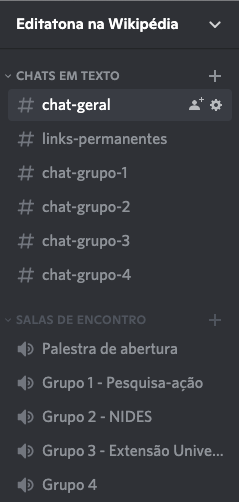
\includegraphics[width=0.5\textwidth]{Images/discord_channels.png}
    \caption{Estrutura das salas criadas no servidor “Editatona na Wikipédia” no Discord.}
    \label{fig:estrutura_discord}
\end{figure}

 O dinamismo possibilitado pelo Discord nos deixou esperançosos, e partimos para a criação e personalização de um servidor lá para nossas atividades. Criamos inicialmente cinco salas multimídias, que na interface do sistema rebatizamos de “Salas de encontro”. A primeira chamada “Palestra de abertura”, onde todos os participantes deveriam se encontrar no início da atividade, e as salas seguintes com nomes como “Grupo 1”, com o numeral sendo incrementado a cada sala nova.
 
 Para as salas de texto, chamadas na interface de “Chats em texto” criamos inicialmente seis. Uma com o mesmo nome de cada grupo, uma intitulada “chat-geral” e por fim uma chamada “links-permanentes”, onde somente o organizador poderia enviar mensagens.
 
 Em torno desta estrutura foi criada a seguinte metodologia para desenvolvimento da atividade: todos os usuários, nos convites enviados para a atividade, foram orientados a entrar na sala “Palestra de abertura” assim que acessassem o servidor. Lá, o wikipedista experiente faria uma apresentação de no máximo meia hora sobre a Wikipédia, introduzindo suas políticas editoriais e a interface do sistema MediaWiki. Após a apresentação, os usuários seriam convidados a acessar o chat “links-permanentes”, clicarem em “Criar uma conta”, e depois informarem no “chat-geral” seu nome de usuário.
 
 Vencido o primeiro contato com a Wikipédia, os participantes então eram convidados a acessar a página criada para organizar os esforços daquela editatona, com link disponível no chat “links-permanentes”. Nessa página, os participantes encontrariam uma lista com sugestões de verbetes a serem trabalhados, lista esta preparada previamente pelo wikipedista experiente e por um representante do grupo que participa da editatona.
 
 Todos são então convidados a debater, em voz ainda na sala “Palestra de abertura” ou em texto no “chat-geral” para os que não puderem/quiserem utilizar microfone, sobre a lista proposta de verbetes a serem trabalhados, que se apresenta apenas como uma sugestão inicial e pode ser totalmente alterada pelos participantes.

\begin{figure}[H]
    \centering
    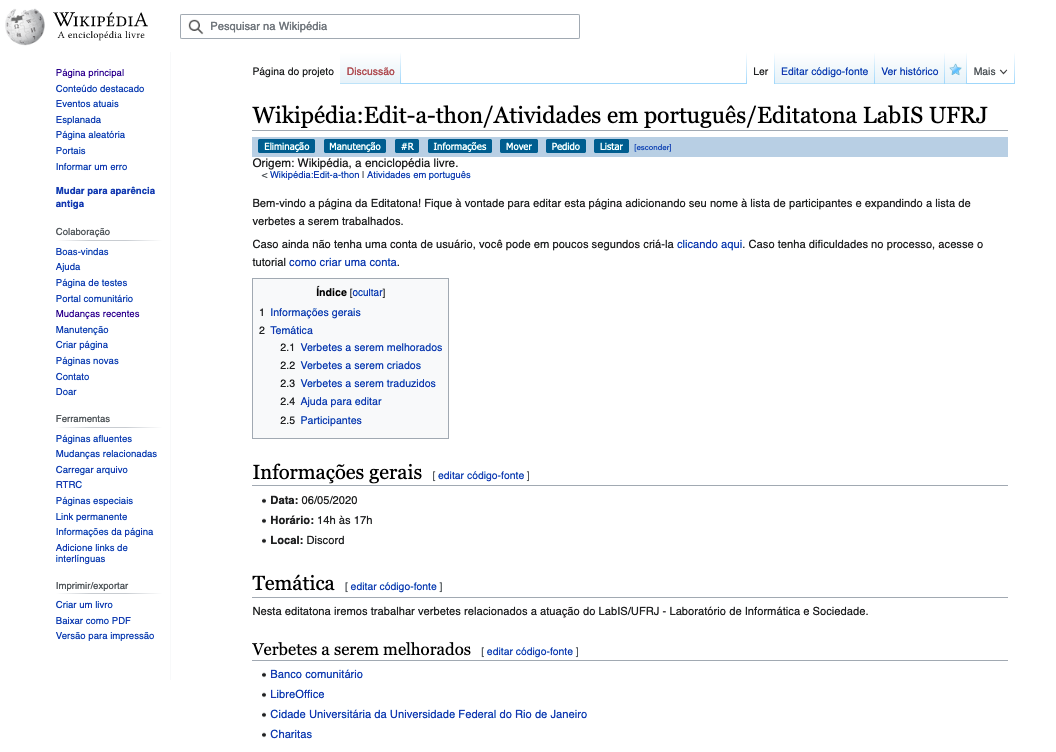
\includegraphics[width=1\textwidth]{Images/pagina_editatona.png}
    \caption{Página de organização de uma das editatonas realizadas durante a pesquisa com lista prévia de sugestões de verbetes a serem melhorados.}
    \label{fig:pagina_editatona}
\end{figure}

 Feita a discussão de quais temas serão trabalhados, o wikipedista experiente então edita o nome das salas que seguiam o padrão ``Grupo X'', adicionando em seus títulos quais temas serão trabalhados em cada sala. Os participantes são então convidados a clicarem no grupo que desejarem, e a sala ``Palestra de abertura'' é esvaziada.
 
 Neste momento começa de fato a escrita enciclopédica, e o wikipedista experiente passa a rodar entre os grupos para auxiliá-los. O MediaWiki, software que gerencia a Wikipédia, não possui funcionalidades que apoiem a escrita ao vivo de textos por duas pessoas que estejam em máquinas diferentes. Isto não é um problema para editatonas presenciais, onde os novatos compartilham o mesmo teclado, mas para a atividade virtual seria muito desmobilizante pedir para um usuário esperar outro editar e salvar uma página de testes para somente então poder editar também. Assim, para dar conta da escrita coletiva em computadores distintos, os grupos recebem a sugestão de utilizar a ferramenta Etherpad para a escrita coletiva de seus rascunhos, antes de passá-los para as páginas de Testes da Wikipédia. 
 
O Etherpad é um software livre que oferece a possibilidade de usuários criarem simultaneamente textos online. Seu funcionamento guarda muitas similaridades com a ferramenta Google Docs, já amplamente conhecida por usuários da Internet. (ARRINGTON, 2008) Optamos por sugerir aos participantes das editatonas a utilização do Etherpad, e não da ferramenta da Google, por ele ser mais leve e não requerer autenticação dos usuários, permitindo que com um apenas um clique o usuário já esteja no ambiente de edição sem maiores burocracias.

Assim, para dar sequência ao trabalho, o usuário experiente cria um pad (nome de uma página dentro do Etherpad) para cada grupo, e compartilha o link de cada um no chat de texto dentro do servidor do Discord de cada respectivo grupo.

\begin{figure}[H]
    \centering
    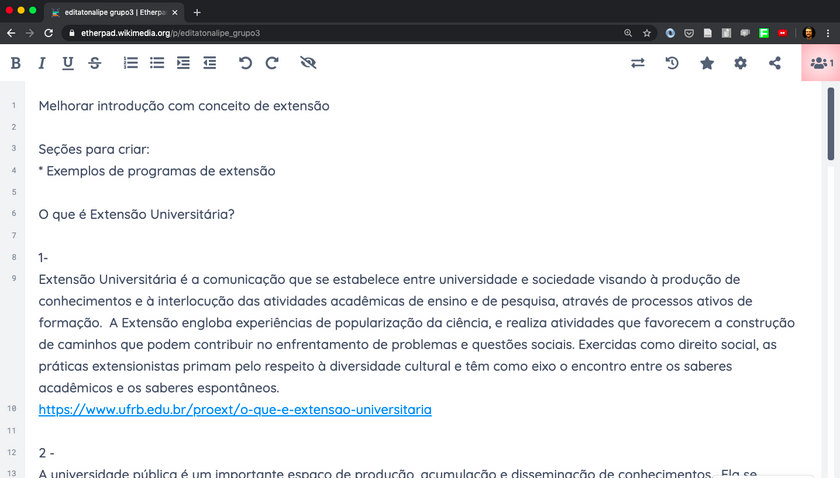
\includegraphics[width=1\textwidth]{Images/etherpad.png}
    \caption{Exemplo de um pad utilizando por um grupo durante uma editatona virtual.}
    \label{fig:etherpad}
\end{figure}

Os membros de cada grupo então são convidados a seguir o seguinte método: escrever no pad o rascunho do texto que irá para a Wikipédia e compartilhar no chat de texto do grupo no Discord links que possam ser utilizados como referências e demais conteúdos relacionados ao processo de escrita do grupo. Desta forma, além do trabalho do grupo ficar estruturado, participantes de todos os grupos poderão acompanhar com facilidade o que estiver acontecendo em cada grupo, possibilitando colaboração e até mudanças de grupo com facilidade se desejarem.

\begin{figure}[H]
    \centering
    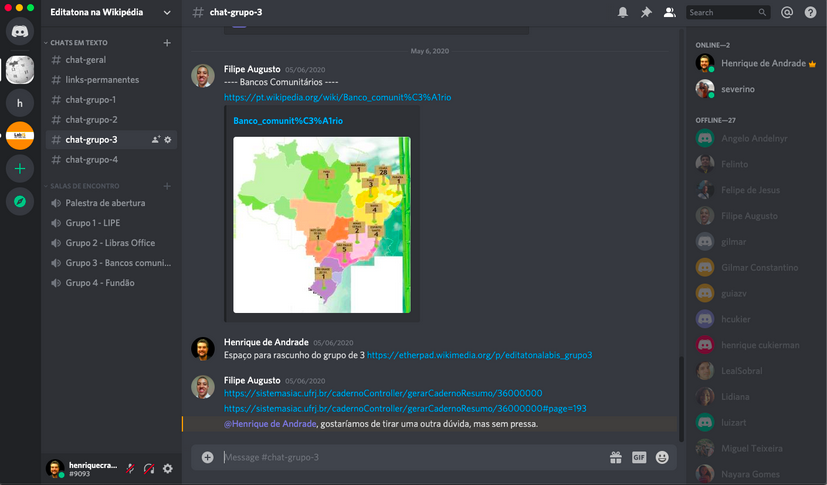
\includegraphics[width=1\textwidth]{Images/discord_full.png}
    \caption{Chat em texto de um grupo das editatonas virtuais, onde podem ser vistos o link para o pad sendo compartilhado e posteriormente um participante pedindo a presença do wikipedista experiente.}
    \label{fig:discord_chat}
\end{figure}

Os grupos são também orientados a utilizar, sempre que desejarem, a ferramenta de ``marcação'' do Discord para chamar o wikipedista experiente. Em qualquer sala de texto, ao digitar o carácter ``@'' seguido do nome de um usuário, ele recebe uma notificação da ferramenta. Assim, o coordenador da atividade, que pode estar na sala de outro grupo, poderá com facilidade saber que um grupo precisa de ajuda, e se dirigir a ele imediatamente com um simples clique.

Após duas horas de produção de conteúdo, o wikipedista experiente roda todos os grupos uma última vez, os auxiliando a salvar seus conteúdos e convidando todos os participantes a retornarem para a sala "Palestra de abertura", onde é realizado um bate-papo final com todos, com cada grupo contando para os demais o que foi produzido, relatando como foi a experiência e narrando quais dificuldades encontraram no processo.

Com um novo roteiro definido para dar conta do novo contexto, partimos então novamente para a fase da pesquisa onde realizaríamos editatonas, só que agora virtualmente.